\documentclass[11pt, a4paper, oneside]{article}

% Packages
\usepackage{fullpage}			% fullpage margins
\usepackage{graphicx, float}		% for graphics/figures
\usepackage{amsmath, amssymb}	% math formatting and symbols
\usepackage{color}
\usepackage{enumerate}
\usepackage{hyperref}
\usepackage{parskip}
\usepackage{setspace}

\onehalfspacing

% Environment for theorems
\usepackage{amsthm}			% http://www.ctex.org/documents/packages/math/amsthdoc.pdf
\newtheorem{lem}{Lemma}

\begin{document}
\pagenumbering{roman}
% Title
\title{CS4246 Project Report\\ Monte Carlo Tree Search in Texas Hold'em Poker}
\author{Choo XianJun, Davin [A0092084E] \\ Lim Keng Kiat [A0087026E] \\ Wang Zi [A0105682H]}
\date{} % Blank out the date
\maketitle

\tableofcontents

\section{Introduction}
\pagenumbering{arabic}
\subsection{Background}
As part of the course requirement\footnote{CS4246 AI Planning and Decision Making}, our group chose to work on a survey project. In this project option, we were to read up several related papers on a chosen theme and write a coherent survey of the topic.

The choice of topic of our group is Monte Carlo Tree Search. The decision of looking into a Monte Carlo method is two fold. Firstly, many real world problems are inherently complex and a clean, exact solution is either hard to formulate or computationally prohibitive. Secondly, techniques such as Monte Carlo Tree Search are very general and have applications in various domains, as long as we are able to see the link and formulate the problem properly.

\subsection{Organisation of report}
In this report, we will first share our findings about Monte Carlo Tree Search - what it is, interesting subproblems and common extensions. Next, we look at the problem domain of Texas Hold'em Poker to gain some hands-on experience on the topic. Lastly, we discuss some observations from our implementation of a Monte Carlo Tree Search Poker bot.

\section{Monte Carlo Tree Search}
\subsection{Overview}
Monte Carlo Tree Search (MCTS) is a heuristic tree search algorithm.

The concept of random sampling is the soul of Monte Carlo techniques. An example would be Monte Carlo integration where random samples are used to approximate the area or volume of an object of interest. The key reason why Monte Carlo methods work is because as the number of random samples increase, the approximate converges towards the true value.

In similar fashion, MCTS employs random sampling to perform approximate search on a large tree. In classic tree search algorithms, such as $\alpha$-$\beta$ pruning or $A^*$ search, we usually need to provide a evaluation function for intermediate/non-terminal states. This evaluation function may be hard to derive or unwieldy to compute. MCTS circumvents this by removing the need of such a function - it only needs to be able to evaluate the terminate states. As such, MCTS is \textit{aheuristic}.

Another advantage of MCTS over the classical tree search algorithms it is an \textit{anytime} algorithm. That means we can terminate a MCTS run at any time and still yield a reasonable solution (as opposed to its counterparts which do not yield any meaningful solution if terminated halfway through computation).

MCTS also performs \textit{asymmetric} tree search which favours more promising nodes instead of uniformly exploring all possibilities. This reallocation of precious computation time helps to improve the approximation performance of MCTS. \autoref{fig:asymmetric} illustrates the search tree of one of the simulation instance from our MCTS Poker bot.

\begin{figure}[H]
	\centering
	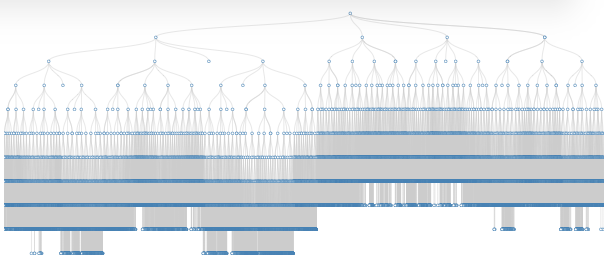
\includegraphics[width=0.75\textwidth]{asymmetric.png}
	\caption{Illustration of asymmetric search tree of our MCTS Poker bot}
	\label{fig:asymmetric}
\end{figure}

These are a few reasons why MCTS is gaining popularity over its classical counterparts in areas such as artificial intelligence in games.

MCTS comprises of 4 phases in a given sampling step, as shown in \autoref{fig:MCTS}. These steps are repeated either for a fixed number of times or until it runs out of computation time.

\begin{figure}[H]
	\centering
	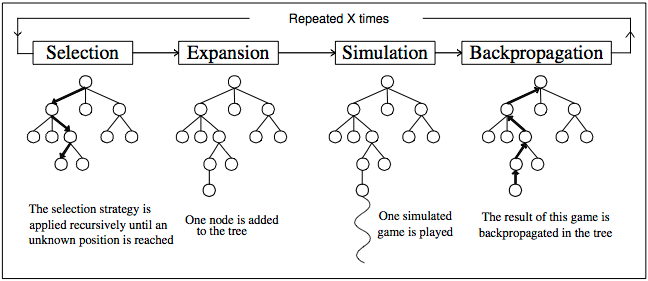
\includegraphics[width=0.75\textwidth]{MCTS_outline.png}
	\caption{Monte Carlo Tree Search outline from ~\cite{Chaslot2010}}
	\label{fig:MCTS}
\end{figure}

\subsection{The 4 Phases}
\subsubsection{Selection}
In this step, we perform what some references call the ``Tree Policy'' ~\cite{Browne2012}. This steps occurs when we are at a node whose available actions have all been explored at least once before. Here, we make a decision which of the child nodes to explore. Among several methods, the most popular ones are Upper Confidence Bound (UCB1) and Upper Confidence Bound for trees (UCT), which we will discuss later. More complicated MCTS implementations can also incorporate some kind of opponent modelling into this phase. We will see more on the topic of opponent modelling and adaptive play later on.

\subsubsection{Expansion}
Once we reach a node where not all available actions have been explored, we choose between one of the unexplored ones to expand the search tree. A common way to do so is just to pick uniformly across all remaining unexplored actions.

\subsubsection{Simulation}
Some references refer this step as ``Default Policy'' ~\cite{Browne2012}. From this step onwards, every node is new to the search tree. The vanilla simulation step would be to uniformly pick among all possible actions at each node and play out the search tree until it hits a terminal node. Similar to the ``Selection'' phase, opponent modelling can also be incorporated in this phase.

\subsubsection{Backpropagation}
Lastly, once we hit a terminal node, we will evaluate the terminal node and do some book-keeping. By that, we mean we update information in the all nodes involved in this iteration of random sample. What is updated would depend on what is needed in the implementation of MCTS. For example, to implement UCB1/UCT, we need to update the heuristic value of each node from the terminal node to the root, and the number of times we have explored each node of these nodes in all iterations so far.

\subsection{Exploration vs. Exploitation}
The problem of exploration versus exploitation frequently encountered in the field of decision making. A typical scenario would be one where we have to decide whether to continue making choices that have been giving good results or take risks to try things that we have little empirical evidence for, in hopes that we might discover better options. In particular, during the ``Selection'' phase of MCTS, our decision for picking a child node is in fact a problem of exploration versus exploitation. In this section, we explore the two most popular methods of tackling this issue: Upper Confidence Bound (UCB1) and Upper Confidence Bound for Trees (UCT).

\subsubsection{Upper Confidence Bound}
Upper Confidence Bound (UCB1) came from the literature of the multi-arm bandit problem. The setting for the multi-arm bandit is as follows: In a casino, there are several slot machines\footnote{A slot machine is also known as one-armed bandit}, each with an unknown probability of giving the player a reward. A player is then supposed to maximize their reward over $N$ plays. Since the probabilities are unknown, players need to trade off exploration (try different slot machines) and exploitation (keep pulling the slot machine that gave him/her the most amount of reward so far).

Regret minimization is often employed in this scenario. Regret is defined as the expected loss due to not playing the optimal slot machine. In economics sense, one can also view it as the opportunity cost. Note that in reality, the player does not know which is the best bandit while making decisions.

In light of this, it is helpful to have some sort of confidence bound that a given slot machine is optimal. ~\cite{Auer2002} proposed the following Upper Confidence Bound policy:

$$UCB1 = \overline{X}_j + \sqrt{\frac{2\ln n}{n_j}}$$
$$
\begin{array}{rrcl}
\text{where}  & \overline{X}_j & : & \frac{v_j}{n_j}\\
              & n & : & \text{Number of times we visited the current/parent node}\\
              & n_j & : & \text{Number of times we visited the child node $j$}\\
              & v_j & : & \text{Heuristic value of the child node $j$.}\\
              & & & \text{Usually a sum of rewards across all simulations.}\\
\end{array}
$$

At each ``Selection'' phase of the MCTS, we simply pick the child node that maximizes the UCB1 value.

\subsubsection{Upper Confidence Bound for Trees}
Upper Confidence Bound for Trees (UCT) is a variant of UCB1 with a slight modification that allows more control over how much to favour exploration over exploitation:

$$UCT = \overline{X}_j + 2C_p\sqrt{\frac{2\ln n}{n_j}}$$
$$
\begin{array}{rrcl}
\text{where}  & \overline{X}_j, n, n_j & : & \text{Same as UCB1}\\
              & C_p & : & \text{A constant greater than 0}\\
\end{array}
$$

~\cite{Kocsis} showed that a value of $C_p = \frac{1}{\sqrt{2}}$ satisfies the Hoeffding inequality with rewards in the range of $[0,1]$.

\subsection{Extensions to MCTS}
\subsubsection{Parallelization}
In today's scenario where devices are granted multiple cores but individual core processing speeds are stagnating, there is merit in parallelizing MCTS. We show the 3 main ways of doing so below.

\textbf{Leaf parallelization}
At the beginning of the ``Simulation'' phase, starting at the leaf node, for each available thread, spawn a simulation all the way until terminal nodes, and then backpropagate the results back up.

\textbf{Root parallelization}
Build multiple MCTS trees and run them in parallel separately. They do not communicate or interfere with each other. At the point in time when a decision is to be made, select the best move from the consolidated results of all the MCTS trees.

\textbf{Tree parallelization}
Have several threads run on a single MCTS tree. In this case, we need to use mutexes to lock up certain parts of the tree to prevent data corruption.

\textbf{Comparisons}
Of the three methods, leaf and root parallelizations are easier to implement while tree parallelization requires more care due to the potential data corruption. ~\cite{Chaslot} suggests that the root and tree parallelizations perform better than leaf parallelization.

\subsubsection{Re-using simulation branches}
Since MCTS is an approximate method that attains better performance as the number of simulations increase, an obvious way is to re-use certain appropriate simulations that have been conducted before. For example, in the root node, we have $K$ child nodes. After running a few iterations of MCTS, a decision is made to visit the child node $j$. The vanilla MCTS would toss away the entire tree and restart the process from scratch by setting node $j$ as the root. Instead of that, we could toss away everything while retaining the branch that has node $j$ as the root. By doing so, we start off the next round of MCTS with ``free'' simulations from the previous step. This will help improve the optimality of the MCTS approximation.

\subsubsection{Opponent Modelling}
One of the drawbacks of pure MCTS is that it tries to run simulations with no regards to the opponent's hands. Therefore, it tends to run excessive simulations on actions that are not necessary such as simulating the possibilities of a high raise given a weak hand. Assuming that the opponent is playing rationally, it may be better to try and guess what possible hands that the opponent currently has given the action history so that one can make a better play. For example, an opponent that plays aggresively after the flop may suggest a stronger hand, therefore the agent can rule out possibilties of all possible card combinations that result in a weak hand. This increases the efficacy of each simulation in the MCTS process.

In addition, there has been research, such as ~\cite{Maitrepierre} on adaptive play opponent modelling techniques. This is useful if the opponent were to change his/her strategies over time (Player that has been playing tightly suddenly decides to play loosely). Adaptive play learns a table of the usual moves that the opponent make for each class of card combinations in their hands (e.g. deuces, high card, etc) and will start the re-learning process if it detects that the current play is significantly different from the learned table.

\section{Texas Hold'em Poker}
\subsection{Terminologies and rules}
For the sake of this assignment, we had to impose certain assumptions about the game so as to reduce the scope of our problem, and make it tractable. Thus, we have scoped the game as a Two-player Limit Texas Hold'em Poker game. We do so to greatly simplify the MCTS tree that needs to be simulated. However, the MCTS algorithm can, in principle, be generalise to any number of players, at a cost of requiring more simulations. In addition, we have assumed that in Limit Poker, all raises and bets have been discretized into either a big bet (e.g. \$20) or a small bet (e.g. \$10). This would greatly simplify the branching required in constructing our MCTS tree. When playing against a human, any bets taken greater than or equal to $x$ will be treated as a big bet action, and likewise, any bets lower than $x$ will be taken as a small bet action.

A Texas Hold'em game can be described as four distinct stages, Deal, Flop, Turn and River. 
First, each player is dealt 2 hidden cards that is not shown to the other players. It is followed by a betting round where each player places their bets. The stage only proceeds when all the players has either matched their bets with one another, or has folded. 
Next, 3 community cards are dealt in the flop stage, and again, a betting round commences. In the Turn and the River stages, 1 card is added in each stage to community cards, separated by a betting round.

At the end of the final betting round (after the river), the cards of the remaining players are revealed. The player with the best card combination taken from his/her hand an the 5 community cards wins the game. \autoref{fig:Poker hand strength} shows the strength of Poker hands in descending order.

\begin{figure}[h!]
\centering
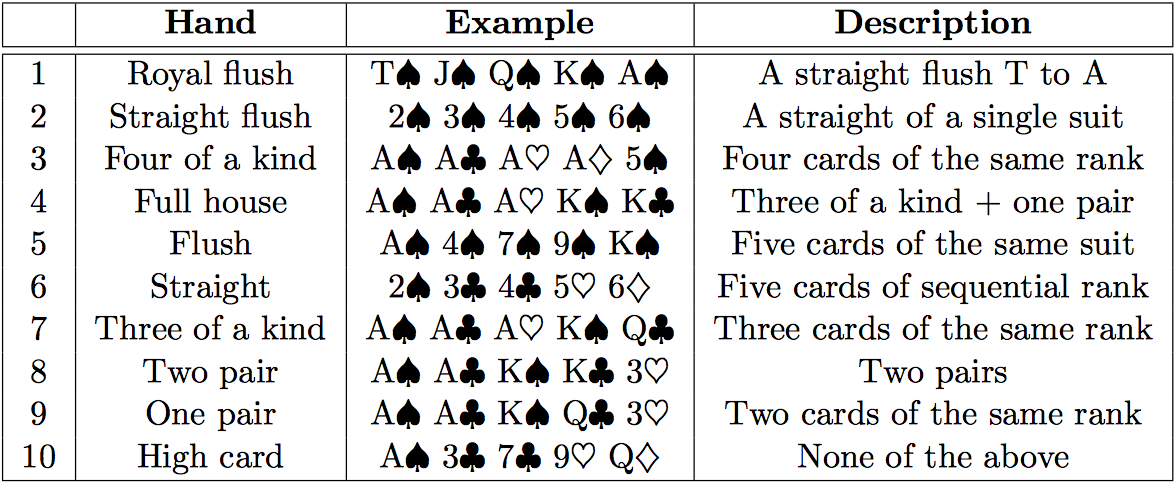
\includegraphics[width=\textwidth]{pokerhand.png}
\caption{Poker hand strength from ~\cite{Kleij2010}}
\label{fig:Poker hand strength}
\end{figure}

\subsection{Poker as a problem domain}
\textbf{Characteristics of the game}
The game of Poker is an interesting problem to look at with respect to decision making.

In Poker, there is imperfect information, which translates to a huge state space. At any point, due to partial observability\footnote{We cannot observe the opponent's hand}, there will be many possible states that the game might be in. This immediately reduces the effectiveness of simple brute force search methods.

Another interesting property of Poker is the fact that there are non-deterministic outcomes to decisions made by players. This happens in the form of the cards dealt by the dealer (either to players or to the community pool). As such, we need to assimilate that random factor into our decision making.

\textbf{Alternative approaches}
Prior to the rise of popularity of MCTS, the most common approach to solving Poker games was via Game theory ~\cite{Johanson2007}, ~\cite{Sandholm2010}. The methods generally formulate Poker into a two player game and attempts to solve the Nash equilibrium. However, due to the large number of leaves in the game tree, it is computationally prohibitive to compute the Nash equilibrium. As a result, plenty of work has been done to optimize computation and find suitable approximations to the original Poker game tree. Unfortunately, even with approximation methods, it may still takes months to solve the Poker game\footnote{In ~\cite{Sandholm2010}, it was mentioned that ``approximate equilibrium finding takes months on a shared-memory super-computer using 96 cores.''.}.

\section{Implementation}
Using Python 2.7, we implemented a poker bot using the MCTS algorithm\footnote{Source code is available here: \url{https://github.com/sozos/MCTS}}. This is done on the Poker Armageddon simulator. This has allowed us to concentrate fully on implementing the bot, without worrying about the intricate details of the rules of the game (all-in conditions can be cumbersome to implement).

\autoref{fig:bot} shows a sample execution of our program via the command \texttt{python main.py <Player 0> <Player 1>}. A \texttt{human\_bot} is a stub used to ask inputs from the human player.

\begin{figure}[h!]
\centering
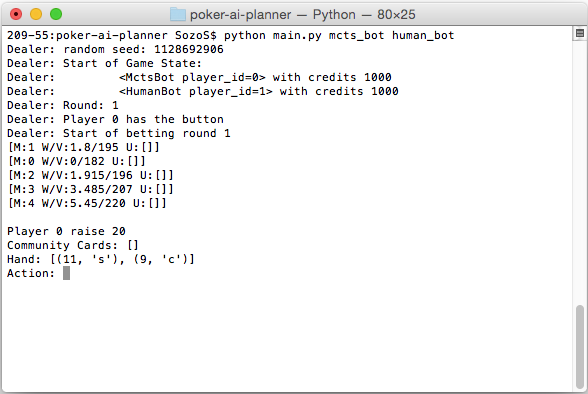
\includegraphics[width=\textwidth]{bot.png}
\caption{Screenshot of our MCTS bot}
\label{fig:bot}
\end{figure}

The standard MCTS algorithm proved to be rather straightforward. However, there were a few elements that we had to customize for our poker game. Firstly, we had to decide how should the simulations be cut off. Typically, an MCTS can be cut off either by the number of simulations run, or by timing. For the sake of simplicity, and to avoid other unpredictable factors that could creep in due to OS scheduling problems, we have decided to limit the simulations to 10,000.

Naturally, the more simulations are run, the better the MCTS bot gets at making decisions. However, the tradeoff is the time taken for the computations. In most poker games (especially online), there is a time limit to make decisions, and running long simulations may not be possible. However, we have empirically found that the actions between a bot that runs simulations in the order of 10,000 tend not to deviate much from that in the order of 100,000 and beyond. As such, we have decided that 10,000 is sufficent enough to make good betting calls.

Secondly, we have to choose a proper reward function for the game such that MCTS would be able to properly assimilate the results from the simulations into the scoring for each actions. We have decided that our reward functions returns the total number of credits (chips) that the agent will end up with after the game. This is because of the theoretical properties of UCB1 and UCT are for rewards in the range of $[0,1]$.

It is interesting to note that the performance of the bot greatly depends on the reward function used. Initially, we have tried to use a reward function that returns the winnings of the game for the winner, and \$0 for the loser. This makes common sense, since in an episodic game, that is what an agent should optimise for. However, when we run the simulations, we found out that our agent has a very high tendency to play aggressively and take high raises. We realised that our agent failed take incorporate the risks taken for each action - although high raises increases the potential reward, it also increases the potential losses. A reward of \$0 for the loser simply did not account for such risks.

Therefore, a reward function that returns the total number of credits each player has gotten (depending on whether they have won or lost) seems apt enough to account for both the risks, and the reward.


\section{Conclusion}
The project was a fruitful one. We learnt about a new decision making technique - Monte Carlo Tree Search., and useful extensions of it. It's generality allows us to apply what we have learnt into other problem domains besides Poker. We expect to see further applications beyond the course.

But perhaps the key takeaway for us would be learning the difference between theory and practical implementation. It is one thing to understand the algorithm and it's theoretical results, and yet another to implement it to solve a specific problem. To do so, one would have to abstract the problem correctly and then encode it into the form that the algorithm accepts. After which, we have to make sense of the output of the algorithm by decoding back to the problem domain. This lesson would not have happened if we did not try to implement what we have learnt about MCTS into our Poker bot. Hence, we are grateful for the opportunity to do so.

\newpage
\bibliography{report}{}
\bibliographystyle{ieeetr}

%{\color{red}Write bibtex and fix references}
%[1] Chaslot's Thesis
%[2] Browne et al: A Survey of Monte Carlo Tree Search Methods: http://www.cameronius.com/cv/mcts-survey-master.pdf
%[3] http://mcts.ai/about/index.html
%[4] http://homes.di.unimi.it/~cesabian/Pubblicazioni/ml-02.pdf
%[5] Michael Bradley Johanson: Robust Strategies and Counter-Strategies: Building a Champion Level Computer Poker Player
%[6] Tuomas Sandholm: The State of Solving Large Incomplete-Information Games, and Application to Poker
%[7] Chaslot et al: Parallel Monte-Carlo Tree Search: https://dke.maastrichtuniversity.nl/m.winands/documents/multithreadedMCTS2.pdf
%[8] Kocsis et al.: Improved Monte-Carlo Search: http://www.ualberta.ca/~szepesva/papers/cg06-ext.pdf
%[9] Raphael Maitrepierre et al.: Adaptive play in Texas Hold'em Poker: http://eprints.pascal-network.org/archive/00005142/01/adaptivePlay.pdf
%%%%%%%%%%%%%%%%%%%%%%%%%%%%%%%%%%%%%%%%%%%%%%%%%%

\end{document}